% ─────────────────────────────────────────────────────────────────────────────
% Figure: Age × Gender Effects on Mean AnthroIndex
% Requires: \usepackage{pgfplots}  \pgfplotsset{compat=1.18}
% ─────────────────────────────────────────────────────────────────────────────

\begin{figure}[t]
  \centering
  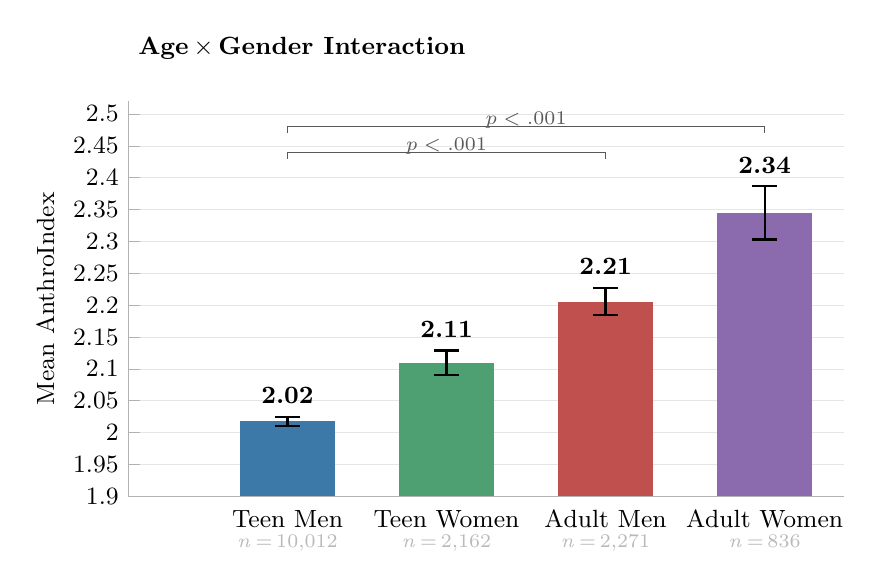
\begin{tikzpicture}
    \begin{axis}[
      width=0.88\columnwidth,
      height=6.6cm,
      clip=false,
      %
      xmin=-0.5, xmax=4.0,
      ymin=1.90, ymax=2.52,
      %
      % No x-axis ticks — we label manually below
      xtick=\empty,
      %
      ytick={1.90, 1.95, 2.00, 2.05, 2.10, 2.15, 2.20, 2.25, 2.30, 2.35, 2.40, 2.45, 2.50},
      yticklabel style={font=\small},
      ylabel={Mean AnthroIndex},
      ylabel style={font=\small},
      %
      ymajorgrids=true,
      grid style={gray!20, very thin},
      axis x line*=bottom,
      axis y line*=left,
      every outer x axis line/.append style={gray!60},
      every outer y axis line/.append style={gray!60},
      tick style={gray!60},
      %
      title={\textbf{Age\,$\boldsymbol{\times}$\,Gender Interaction}},
      title style={font=\small, at={(0.0,1.04)}, anchor=south west},
    ]

      % ── Bars (drawn manually as filled rectangles) ──
      % Bar width = 0.6 data units, centered on x = 0.5, 1.5, 2.5, 3.5

      % Data (from JSON results, RQ2 subgroups):
      %   Teen Men:    M = 2.018, 95% CI [2.011, 2.025], n = 10,012
      %   Teen Women:  M = 2.110, 95% CI [2.091, 2.129], n =  2,162
      %   Adult Men:   M = 2.205, 95% CI [2.184, 2.227], n =  2,271
      %   Adult Women: M = 2.345, 95% CI [2.303, 2.387], n =    836

      % Teen Men (blue)
      \fill[fill={rgb,255:red,60;green,120;blue,168}]
        (axis cs:0.2, 1.90) rectangle (axis cs:0.8, 2.018);
      % Teen Women (green)
      \fill[fill={rgb,255:red,78;green,160;blue,114}]
        (axis cs:1.2, 1.90) rectangle (axis cs:1.8, 2.110);
      % Adult Men (red)
      \fill[fill={rgb,255:red,192;green,80;blue,77}]
        (axis cs:2.2, 1.90) rectangle (axis cs:2.8, 2.205);
      % Adult Women (purple)
      \fill[fill={rgb,255:red,139;green,107;blue,174}]
        (axis cs:3.2, 1.90) rectangle (axis cs:3.8, 2.345);

      % ── Error bars (95% CIs) ──

      % Teen Men: [2.011, 2.025]
      \draw[black, thick] (axis cs:0.5, 2.011) -- (axis cs:0.5, 2.025);
      \draw[black, thick] (axis cs:0.42, 2.011) -- (axis cs:0.58, 2.011);
      \draw[black, thick] (axis cs:0.42, 2.025) -- (axis cs:0.58, 2.025);

      % Teen Women: [2.091, 2.129]
      \draw[black, thick] (axis cs:1.5, 2.091) -- (axis cs:1.5, 2.129);
      \draw[black, thick] (axis cs:1.42, 2.091) -- (axis cs:1.58, 2.091);
      \draw[black, thick] (axis cs:1.42, 2.129) -- (axis cs:1.58, 2.129);

      % Adult Men: [2.184, 2.227]
      \draw[black, thick] (axis cs:2.5, 2.184) -- (axis cs:2.5, 2.227);
      \draw[black, thick] (axis cs:2.42, 2.184) -- (axis cs:2.58, 2.184);
      \draw[black, thick] (axis cs:2.42, 2.227) -- (axis cs:2.58, 2.227);

      % Adult Women: [2.303, 2.387]
      \draw[black, thick] (axis cs:3.5, 2.303) -- (axis cs:3.5, 2.387);
      \draw[black, thick] (axis cs:3.42, 2.303) -- (axis cs:3.58, 2.303);
      \draw[black, thick] (axis cs:3.42, 2.387) -- (axis cs:3.58, 2.387);

      % ── Mean labels above error bars ──
      \node[font=\small\bfseries, anchor=south] at (axis cs:0.5, 2.030) {2.02};
      \node[font=\small\bfseries, anchor=south] at (axis cs:1.5, 2.134) {2.11};
      \node[font=\small\bfseries, anchor=south] at (axis cs:2.5, 2.232) {2.21};
      \node[font=\small\bfseries, anchor=south] at (axis cs:3.5, 2.392) {2.34};

      % ── Group labels below x-axis ──
      \node[font=\small, anchor=north] at (axis cs:0.5, 1.893) {Teen Men};
      \node[font=\small, anchor=north] at (axis cs:1.5, 1.893) {Teen Women};
      \node[font=\small, anchor=north] at (axis cs:2.5, 1.893) {Adult Men};
      \node[font=\small, anchor=north] at (axis cs:3.5, 1.893) {Adult Women};

      % ── Sample sizes below group labels (spaced well below names) ──
      \node[font=\scriptsize, text=gray!55, anchor=north]
        at (axis cs:0.5, 1.855) {\textit{n}\,=\,10,012};
      \node[font=\scriptsize, text=gray!55, anchor=north]
        at (axis cs:1.5, 1.855) {\textit{n}\,=\,2,162};
      \node[font=\scriptsize, text=gray!55, anchor=north]
        at (axis cs:2.5, 1.855) {\textit{n}\,=\,2,271};
      \node[font=\scriptsize, text=gray!55, anchor=north]
        at (axis cs:3.5, 1.855) {\textit{n}\,=\,836};

      % ── Significance brackets ──
      % Teen Men vs Adult Men
      \draw[black!65, thin]
        (axis cs:0.5, 2.43) -- (axis cs:0.5, 2.44)
        -- (axis cs:2.5, 2.44) -- (axis cs:2.5, 2.43);
      \node[font=\scriptsize, text=black!65]
        at (axis cs:1.5, 2.45) {$p < .001$};

      % Teen Men vs Adult Women
      \draw[black!65, thin]
        (axis cs:0.5, 2.47) -- (axis cs:0.5, 2.48)
        -- (axis cs:3.5, 2.48) -- (axis cs:3.5, 2.47);
      \node[font=\scriptsize, text=black!65]
        at (axis cs:2.0, 2.49) {$p < .001$};

    \end{axis}
  \end{tikzpicture}

  \caption{Mean AnthroIndex by age group and gender ($N = 15{,}281$ users
    with $\geq 0.60$ classifier confidence). Error bars show 95\% confidence
    intervals. Both age ($d = 0.50$, adults higher) and gender
    ($d = 0.29$, women higher) were significant predictors, with a
    significant interaction ($p = .013$).}
  \label{fig:age-gender-effects}
\end{figure}
